\section{Payment}

Payment er den widget der er blevet implementeret til sidst i projektet, hvilket har fordele og udlemper. Den teoretiske vidne om projektet har på daværende tidpunkt været bedre end i starten af udviklingsperioden. Derfor består Betaling af en del client-side kode, som skulle forbedre brugervenligheden af widget'en. 

\subsection{Design}
Betaling er som nævnt i Arkitektur-afsnittet blevet designet med inspiration fra MobilePay's underafdeling, WeShare. Det skulle dermed være muligt at splittet en regning mellem alle brugere. Designmæssigt tager Betaling samme struktur som List, hvor der er brugt endnu et PartialView for at liste alle betalere. Derfor kan list demonstreres ud fra nedenstående diagram, der viser kompositionen mellem et view der bliver dannet af andre views.

\begin{figure}[H]
    \centering
    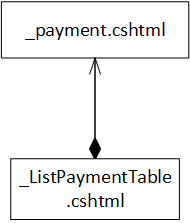
\includegraphics{10_Design_og_implementering/Payment/Images/Betaling_Composition.png}
    \caption{Designmæssigt er en Betaling bestående af 2 PartialViews. \_ListPaymentTable bliver brugt til at liste alle betalere, hvilket giver en bedre seperation of concern, da det giver et bedre overblik for det visuelle.}
    \label{fig:my_label}
\end{figure}

Ydermere består Betaling af et popup vindue, der sørger for at bruger kan tilføje en ny udgift til en eksisterende Betaling.

\subsection{Implementering}

Implementeringsmæssigt er Betaling end med at bestå af 3 controller actions, som bliver kaldt gennem AJAX. Den ene sørger for at accepterer en betaling, hvilket godt kunne blive gjort anderledes. På nuværende tidspunkt bliver en betaling "accepterert" ved at blive slettet fra betalingen. Det ville i fremtidige itterationer være at foretrække hvis betalingen ikke blev slettet, men i stedet blev vist med fx. et flueben.\\

\noindent Det er i Payment muligt at folde widget'en ud, så man både kan se et overblik over alle betalere, men også kun se de første 3 betalere. Dette kan skabe godt overblik på Dashboard for en gruppe. Alternativt kunne der blive taget brug af popup vinduer, der kunne vise alle betalere, og derfra redigerer status.\\

\noindent Implementering for at tilføje en ny udgift til en betaling, er endt med kun at gøre så ejeren kan gøre dette. Det kunne skabe lidt problemer i forhold til hvem der er ejer af betalingen og gerne vil kunne acceptere udgifter. Dette ville helt sikkert godt kunne gøres anderledes i fremtidige itterationer.\\

% \noindent DAL for Betaling bliver brugt til at bredde koden endnu mere ud, selvom MVC i forvejen giver god separation of concern. Metoderne i Data Access Laget bliver brugt hyppigt brug. For at oprette en Betaling, skal der ligeledes oprettes Betalere, med en del attributter, hvilket potentielt kunne tage lang tid. Det er dog på AU's netværk blevet testet at en Betaling med 11 Betalere ikke tager længere tid at lave end andre widgets.\\

% \noindent Den måde udgifter for brugere bliver vist er gennem plain html, hvor der unikt for Betaling i Controlleren er specificeret at dens CultureInfo for nummer format skal sættes sådan at decimal seperatoren er sat til at bruge punktum. Uden dette blev et beløb vist uden nogen separering, hvilket gjorde 10.05 til 1005.\\

% \noindent I bilag kan der ses et mere specifikt hvordan de forskellige controller actions er blevet implementeret. Bl.a. hvordan forskellen mellem "Accept exp." og "Mark Expense" er lavet ud fra om bruger er ejer eller betaler.